% !TEX root = ../Dokumentation.tex
\subsection{Energieversorgung}

\textbf{Funktionsbeschrieb}\\[0.2cm]
Das autonome Entsorgungsfahrzeug muss mit Energie versorgt werden. Dazu werden Akkumulatoren eingesetzt, welche das Gerät während dem gesamten Einsatz mit Strom versorgen. 
\\[0.2cm]
\textbf{Komponentenbeschrieb}\\[0.2cm]
\begin{figure}[h]
\centering
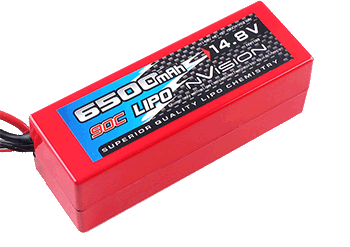
\includegraphics[width=0.5\textwidth]{03_Loesungskonzept/pictures/lipo.jpg}
\caption{2400 mA/h Lipo  (Quelle:http://www.conrad.ch/ce/)}	
\end{figure}\\[0.2cm]
Um Störungen, die z.B durch den erhöten Anlaufstrom der Motoren verursacht werden könnten, zu vermeiden, werden die intelligenten Systeme (Microcontroller, Mini-Computer,etc.)möglichst getrennt von den Motoren gespiesen. Dazu wird einerseits ein 11.1Volt Lithium-Polymer-Akkumulator für die Motoren und andererseits ein 7.4 Volt Lipo für die empfindlichen Systeme  verwendet. Die finale Evaluation der Kapazitäten ist noch nicht abgeschlossen. Die Resultate der aktuellen Berechnungen werden im Verlauf des Kaptiels noch erläutert.
 \\[0.2cm]
\textbf{Begründung}\\[0.2cm]
Die Entscheidung wird damit begründet, dass Lithium-Polymer-Akkumulatoren in einem vielfältigen Sortiment erhältlich sind und damit eine grosse Flexibilität bei der Auswahl ermöglichen. Somit würde sich die Suche nach einem Ersatz bei allfälligen Änderungen vereinfachen. Ausserdem weisen LiPo, im Vergleich zu anderen Akkumulatoren eine wesentlich kompaktere Bauform auf was entscheidend für die Auswahl war. \\[0.2cm]
\textbf{Berechnungen}\\[0.2cm]
Kapazitätenberechnungen:
\begin{itemize}
\item DC-Motor für den Antrieb:
\[
\frac{P*t}{U} -> \frac{73.98W*0.25h}{12V}= 1.54 Ah
\]
\item Servomotor für die Lenkung:
\[
\frac{P*t}{U} -> \frac{3.76W*0.25h}{4.8V}= 0.19 Ah
\]
\item Servomotor für den Arm:
\[
\frac{P*t}{U} -> \frac{2.5W*0.25h}{4.8V}= 0.13 Ah
\]
\item Servomotoren für Kamerabewegung, Greifer und Behälteröffnung:
\[
\frac{P*t}{U} -> \frac{0.814W*0.25h}{4.8V}= 0.042 Ah
\]
\item Mini-Computer:
\[
I*t -> 2A+0.25h = 0.5 Ah
\]
\item Gesamtkapazität:
\[
1.54Ah+0.19Ah+0.13Ah+3*0.042Ah+0.5Ah = 2.53Ah
\]

\end{itemize}
